% !TeX root = ../main.tex

\section{Simulation Study}

\subsection{Data Simulation}

%!% Have you simulated this only once? I think you would want to do this multiple time and present results across simulations, no?

To test the CarHHMM with STFT, 500 separate sequences of 100 marine-mammal dives were simulated. The coarse-scale observations $Y$ were set as the duration of each dive, and the fine-scale observations $Y^*$ were set as one-dimensional acceleration readings simulated at 50 hertz. the specific procedure used to generate data was as follows: 

\begin{enumerate}
	\item 100 dive durations were simulated using an HMM generative model with the following parameters:
	
	\begin{align*}
		&\Gamma = \begin{pmatrix} 0.4 & 0.6 \\ 0.6 & 0.4 \end{pmatrix} & \\
		% 
		&Y_t|X_t \sim \rm{Gamma} & \\
		&\bbE(Y_t|X_t = 1) = 15 s &\bbE(Y_t|X_t = 2) = 60 s \\
		%
		&\bbV(Y_t|X_t = 1) = 25 s^2 &\bbV(Y_t|X_t = 2) = 100 s^2
	\end{align*}
	
	\item Once the dive durations were calculated, for each $t \in \{1, \ldots, 100\}$, dive $t$ was broken into $\lfloor Y_t/2 \rfloor$ 2-second segments (the end of the dive sequence was discarded). Further, each 2-second segment was assigned a behaviour according to a fine-scale Markov chain $X^*_t$, where $X^*_{t,s^*} \in \{1,2\}$ and $s^* \in \{0,1,\ldots,\lfloor Y_t/2 \rfloor\}$. The parameters of the fine-scale behaviour Markov chain were set to be as follows:
	%
	$$\Gamma^{*(1)} = \begin{pmatrix} 0.25 & 0.75 \\ 0.75 & 025 \end{pmatrix} \qquad 	\Gamma^{*(2)} = \begin{pmatrix} 0.75 & 0.25 \\ 0.25 & 0.75 \end{pmatrix}$$
	%
	where $\Gamma^{*(1)}$ was used for dives where $X_t = 1$ and $\Gamma^{*(2)}$ was used for dives where $X_t = 2$
	
	\item For each 2-second segment, the Fourier modes $\hat{Y}^*_{t,s^*}$ were simulated using the following procedure. Note that the $k^{th}$ Fourier mode of $\hat{Y}^*_{t,s^*}$ is denoted as $\hat{Y}^{*(k)}_{t,s^*}$ :
	
	\begin{align*}
    	\hat{Y}^{*(0)}_{t,0} &\sim \mathcal{N} \left(\mu = 0, \sigma^2 = 0.0025 \right) & \\
    	%
    	\hat{Y}^{*(0)}_{t,s^*} &\sim \mathcal{N} \left(\mu = 0.9Y^{*(0)}_{t,s^*-1}, \sigma^2 = 0.0025 \right), & s^* = 1,2,\ldots, \lfloor Y_t/2 \rfloor \\
    	%
    	\hat{Y}^{*(k)}_{t,t^*} &= a_{t,s^*}^{(k)} i\sqrt{b^{(k)}_{t,s^*}}, & k = 1,\ldots,49 \\
	\end{align*}
	\begin{align*}
	    a_{t,s^*}^{(k)} &\sim  \left\{\begin{array}{lr}
    	-1 & \quad w.p. \enspace 1/2 \\
    	1  & \quad w.p. \enspace 1/2
    	\end{array}\right. \\
    	%
    	(b^{(k)}_{t,s^*}|X^*_{t,s^*}  = 1) &\sim {\rm{Gamma}}(1/k^2, 1) \\
    	%
    	(b^{(k)}_{t,t^*}|X^*_{t,t^*} = 2) &\sim \left\{\begin{array}{lr}
    	{\rm{Gamma}}(1/k^2, 1), \quad & k \notin \{1,2\} \\
    	{\rm{Gamma}}(100,1), & k = 1 \\
    	{\rm{Gamma}}(50,1), & k = 2
    	\end{array}\right. 
	\end{align*}

    \begin{align*}
        \hat{Y}^{*(50)}_{t,s^*} &= 0 & \\
    	%
    	\hat{Y}^{*(k)}_{t,s^*}  &= -\hat{Y}^{*(100-n)}_{t,s^*}, & \qquad k = 51,\ldots,99
    \end{align*}
	
	\item Finally, $Y^*_{t,(100s^*+1):(100s^*+100)}$ was set using the inverse discrete Fourier transform of $\hat{Y}^*_{t,s^*}$:
	$$Y^*_{t,(100s^*+1):(100s^*+100)} = IDFT\left(\hat{Y}^*_{t,s^*}\right)$$
		
\end{enumerate}

There are several practical reasons behind this construction. First, $\hat{Y}^*_{t,t^*}$ is anti-symmetric about $\hat{Y}^{*(50)}_{t,s^*}$ so that its inverse Fourier transform is real-valued. $\hat{Y}^{*(k)}_{t,s^*}$ also decays like $1/k^2$ so that $Y^*_{t,t^*}$ remains continuous within a 2-second window. Note, however, that $Y^*_{t,s^*}$ is not continuous \textit{between} windows, as can be seen in figure (\ref{fig:fourier_example}). However, the jumps are not too severe since $\hat{Y}^{*(0)}_{t,s^*}$ and $\hat{Y}^{*(0)}_{t,s^*+1}$ are highly correlated. See figure (\ref{fig:sim_data}) for details.

\subsection{Ground-Truth parameters}

This generative model gives simulated data where the ground-truth of the CarHHMM is known. For the coarse scale, the ground truth is as follows:

\begin{align*}
    \delta &= \begin{pmatrix} 0.5 & 0.5 \end{pmatrix}\\
	\Gamma &= \begin{pmatrix} 0.4 & 0.6 \\ 0.6 & 0.4 \end{pmatrix} \\
	% 
	Y_t|X_t = 1 &\sim {\rm{Gamma}}\left(\mu = 15 s, \sigma = 5 s\right) \\
	Y_t|X_t = 2 &\sim {\rm{Gamma}}\left(\mu = 60 s, \sigma = 10 s\right) \\
\end{align*}

For the fine-scale, we have:

\begin{align*}
    \delta^{*(1)} &= \begin{pmatrix} 0.5 & 0.5 \end{pmatrix} & \delta^{*(2)} &= \begin{pmatrix} 0.5 & 0.5 \end{pmatrix} \\
    %
    \Gamma^{*(1)} &= \begin{pmatrix} 0.25 & 0.75 \\ 0.75 & 025 \end{pmatrix} & 	\Gamma^{*(2)} &= \begin{pmatrix} 0.75 & 0.25 \\ 0.25 & 0.75 \end{pmatrix} \\
\end{align*}

\begin{align*}
    \left(Z^{*(1)}_{t,s^*} | Z^{*(1)}_{t,s^*-1} \right) &\sim \mathcal{N} \left(\phi^*Z^{*(1)}_{t,s^*-1} + \phi^*\mu^*, \sigma^{*2} \right), & \mu^* = 0, \enspace \phi^* = 0.9, \enspace \sigma^{*2} = 0.025 \\
    %
    \left(Z^{*(2)}_{t,s^*} | X^*_{t,s^*} = 1\right) &\sim {\rm{Gamma}}\left(\alpha^{*(1)}, \beta^* \right), & \alpha^{*(1)} = \sum_{k=1}^{\tilde{f}} \frac{1}{k^2}, \enspace \beta^* = 1 \\
    %
    \left(Z^{*(2)}_{t,t^*} | X^*_{t,s^*} = 2\right) &\sim {\rm{Gamma}}\left(\alpha^{*(2)}, \beta^* \right), & \alpha^{*(2)} = 20 + \sum_{k=2}^{\tilde{f}} \frac{1}{k^2}, \enspace \beta^* = 1 \\
\end{align*}
%
The emission distribution of the 2-second average acceleration $Z_{t,s^*}^{*(1)}$ can be reparameterized as an OU process according to Theorem 1:
%
$$dZ^{*(1)}_{t,t^*} = \beta^*(\gamma^* - Z^{*(1)}_{t,t^*})dt^* + \omega^* dW_{t,t^*}$$

$$\gamma^* = \mu^* = 0, \qquad \beta^* = -\frac{\log(\phi^*)}{\Delta t^*} = 0.0229, \qquad \omega^{*2} = \frac{2\sigma^{*2}\log(\phi)}{\Delta t (\phi^{*2}-1)} = 0.006$$

\begin{figure}[!ht]
	\centering
	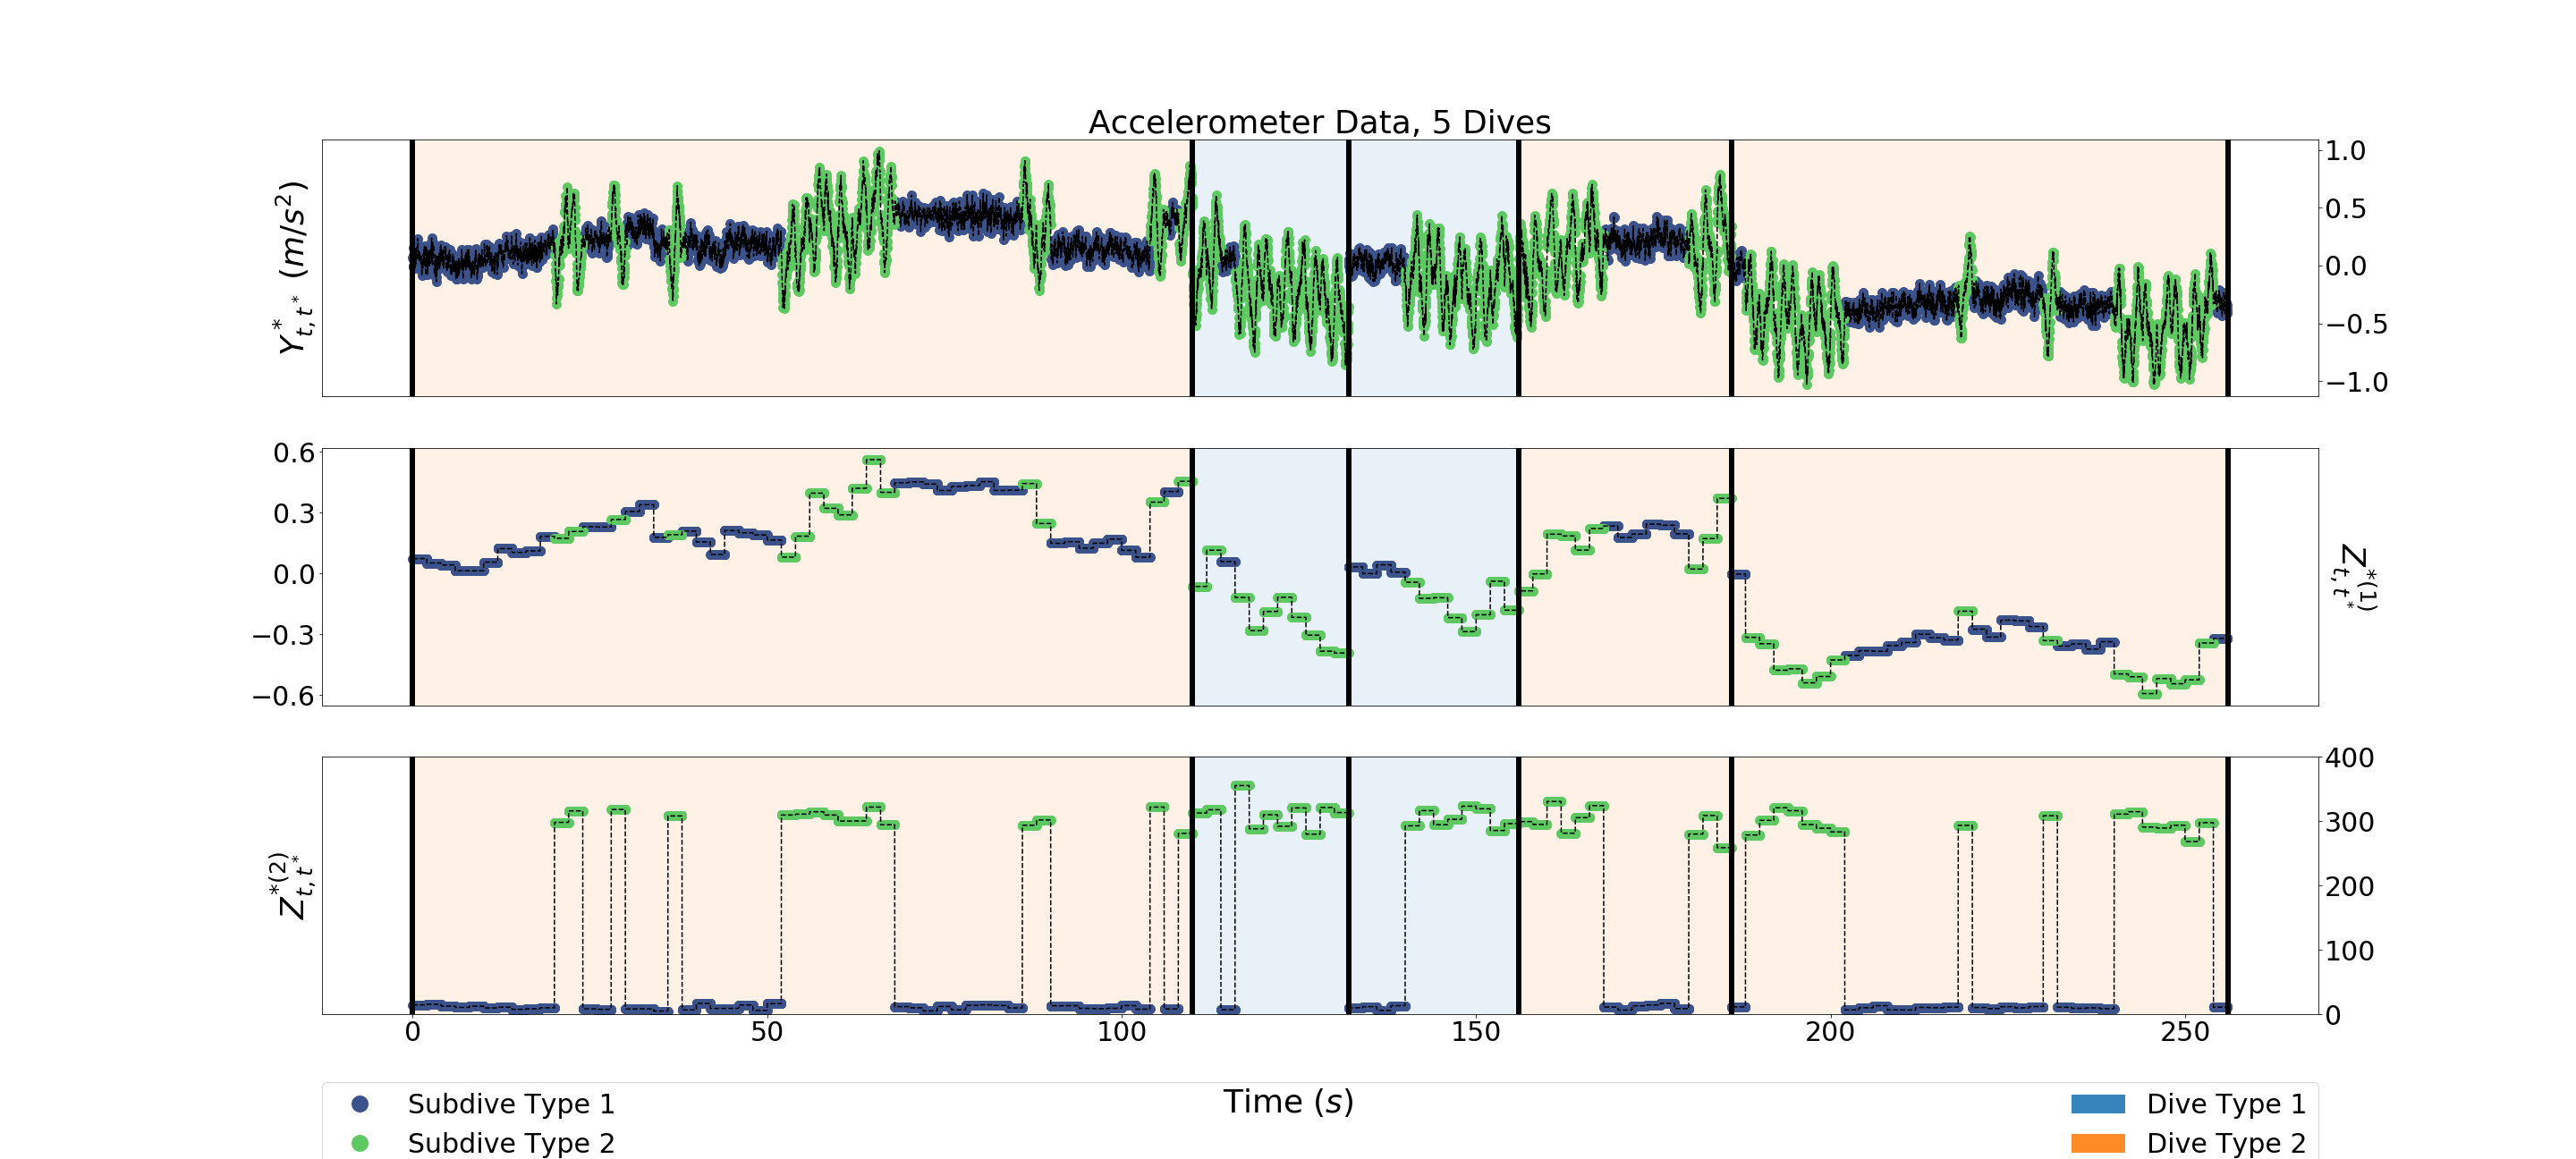
\includegraphics[width=5in]{../Plots/sim_data.png}
	\caption{Simulated Acceleration Data.}
	\label{fig:sim_data}
\end{figure}


\subsection{Simulation Results}

Four different models were fit to each simulated data set:

\begin{enumerate}
    \item A CarHMM with no hierarchical component using both $Z^{(1)}$ and $Z^{(2)}$ as fine-scale observations (CarHMM).
    \item A Hierarchical hidden Markov model with no auto-correlation using both $Z^{(1)}$ and $Z^{(2)}$ as fine-scale observations (HHMM).
    \item A CarHHMM using $Z^{(1)}$, but not $Z^{(2)}$, as fine-scale observations (CarHHMM1).
    \item A CarHHMM using both $Z^{(1)}$ and $Z^{(2)}$ as fine-scale observations (CarHHMM2).
\end{enumerate}
%
For each model, the following were recorded:
%
\begin{enumerate}
    \item An empirical distribution of the MLE estimates of $\Gamma$ and $\Theta$ using the 100 generated data sets generated from true parameters $\Gamma_0$ and $\Theta_0$.
    \item The estimated spread of these distributions using the observed information matrix.
    \item A confusion matrix showing the state decoding capabilities of each model across all data sets.
\end{enumerate}

The empirical distribution of 


%%%%%%%%%%%%%%%%%%%%%%%%%%%%%%%%%%%%%%%%%%%%%%%%%%%%%%%%%%%%%%%%%%%%%%%%%%%%%%%%%%%%%%%%%%%%%%%%


\iffalse
\subsection{Model Misspecification}

There are two ways to simulate the fourier modes of the acceleration vector $\bfA_{s,t}$:

\begin{enumerate}
	\item $$\bbE_1\left(\bfA_{s,t} | \bfA_{s-1,t}, X^*_{s,t}\right) = \phi \bfA_{s-1,t} + (1-\phi) \mu_{X^*_{s,t}} $$
	
	\item $$\bbE_2(\bfA_{s,t} | \bfA_{s-1,t}, X^*_{s,t}, X^*_{s-1,t}) = \left\{\begin{array}{lr}
	\phi \bfA_{s-1,t} + (1-\phi) \mu_{X^*_{s,t}} & \text{for } X^*_{s,t} = X^*_{s-1,t}\\
	\mu_{X^*_{s,t}} & \text{for } X^*_{s,t} \neq X^*_{s-1,t}
	\end{array}\right\}$$
\end{enumerate}

\subsubsection{$\bbE_1$}

First, look at $\bbE_1$. This comes with an issue in that when $X^*_{s,t}$ changes values, it will take a while for the process to ``converge" long-run mean $\mu_{X^*_{s,t}}$. In particular, if the behavioral process $X^*$ had been in state 1 for a while and then switches to state 2 for a while, then:

\begin{align*}
	\bbE_1\left(\bfA_{s+1,t}|X^*_{s:s+1,t} = 2, X^*_{s,t} = 1\right) &=  \phi \mu_1 + (1-\phi) \mu_2 \\
	%
	\bbE_1\left(\bfA_{s+2,t}|X^*_{s:s+2,t} = 2, X^*_{s,t} = 1\right) &= \phi\left( \phi \mu_1 + (1-\phi) \mu_2\right) + (1-\phi)\mu_2 \\
	&= \phi^2 \mu_1 + (1-\phi^2) \mu_2\\
	%
	\bbE_1\left(\bfA_{s+n,t}|X^*_{s:s+n,t} = 2, X^*_{s,t} = 1\right) &=  \phi^n \mu_1 + (1-\phi^n) \mu_2 \\
\end{align*}

So, if using $\bbE_1$, there is an assumption that the fourier modes of the acceleration vector $\bfA$ linearly ``converge" to the new value $\mu_i$ from $\mu_j$ when $X^*_{s,t}$ changes from $i$ to $j$. An example of this can be seen in figure (\ref{fig:FOVEDBA}).

 \begin{figure}[h!]
 	\centering
 	\includegraphics[height=3in]{../Code/test.png}
 	\caption{The FoVeDBA of simulated data using $\bbE_1$. Note that the FoVeDBA approaches $\approx$ 300 in state 2 from $\approx$ 10 in state 1 with roughly linear convergence.}
 	\label{fig:FOVEDBA}
 \end{figure}
 
 Note that if the generative model is correlated, but the inference model isn't, then quick jumps between states 1 and 2 can be missed because the chain never ``converges" to the new mean $\mu_i$, as shown in figure (\ref{fig:STATE}).
 
\begin{figure}[h!]
	\centering
	\includegraphics[height=3in]{../Code/test2.png}
	\caption{The probability of being in each behavioral state $X^*_{s,t}$ as estimated by the HHMM. The colors represent the true behavioral state.}
	\label{fig:STATE}
\end{figure}
 
 \subsubsection{$\bbE_2$}
 
Clearly, the model has issues decodeing the behavioral state when the model is misspecified. Therefore, if the true generative process does not have correlation when jumping between states, then it is better to use $\bbE_2$:

$$\bbE_2(\bfA_{s,t} | \bfA_{s-1,t}, X^*_{s,t}, X^*_{s-1,t}) = \left\{\begin{array}{lr}
\phi \bfA_{s-1,t} + (1-\phi) \mu_{X^*_{s,t}} & \text{for } X^*_{s,t} = X^*_{s-1,t}\\
\mu_{X^*_{s,t}} & \text{for } X^*_{s,t} \neq X^*_{s-1,t}
\end{array}\right\}$$

This fixes the issue of having to ``converge" to the new value of $\mu_i$ when jumping to state $i$. However, note that $\bbE_2$ depends upon both $X^*_{s,t}$ and $X^*_{s-1,t}$. This breaks the assumption in the forward algorithm that $\bfA_{s,t}$ depends only on $X^*_{s,t}$. One way to deal with this issues is to introduce a new hidden state $Z^*_{s,t} = (X^*_{s-1,t},X^*_{s,t})$. This fixes the issue, but now $Z^*_{s,t}$ can take one of $s^2$ values instead of $s$. This grows the state space of our model and can make inference harder.
 
 \fi
 
%Figure (\ref{fig:smoothing}) also shows the calculated ODBA as a function of time for one a specific dive. The acceleration exhibits sinusoidal behavior at several points in time which cannot be modeled using HMMs straightforwardly. As a result, the data was split into two-second intervals (100 data points each), and each interval was summarized by the Fourier transform of the ODBA and the velocity at the \textit{end} of the time interval. Velocity was taken at the end of the time interval because the behavior of the whale during the time interval has no impact on the velocity of the whale at the beginning of the time interval. Because velocity is highly correlated with the average acceleration within an interval, the mean was subtracted out of each ODBA time series before the Fourier transform was taken. To reduce the dimension of the ODBA Fourier transform, Fourier coefficients corresponding to frequencies less than or equal to 5 hertz were summed and frequencies above 5 hertz were ignored. One nice property of this process is that it reduces the number of data points by a factor of 100, which drastically speeds up parameter estimation. The optimal length of the time interval over which to take the Fourier transform is a tuning parameter that is difficult to find. An ideal time interval should be long enough give useful Fourier coefficients, but short enough to preserve as much information about the vertical velocity of the animal as possible.

%\subsection{Lag Plot}

%In order to find the appropriate HMM to model whale behavior, a lag plot was made for both velocity and the ODBA fourier sum. The results of doing so are shown in figure (\ref{fig:lag}). Unfortunately, the number of behavioral states is not clear from the lag plot, but it is clear that the velocity exhibits a large degree of autocorrelation. While the ODBA Fourier sum also exhibits some autocorrelation, the relationship is less strong, so autocorrelation was not incorporated in the ODBA Fourier sums emission distribution.